%%%%%%%%%%%%%%%%%%%%% Chapter 10 %%%%%%%%%%%%%%%%%%%%%%%%%%%%%%%%%
% Robust Aggregation: Surviving Byzantine Adversaries
%%%%%%%%%%%%%%%%%%%%%%%%%%%%%%%%%%%%%%%%%%%%%%%%%%%%%%%%%%%%%%%%%
\motto{In open Federated Learning settings, the threat often comes from the clients themselves. A single malicious update can corrupt the entire global model.}

\chapter{Robust Aggregation: Surviving Byzantine Adversaries}
\label{chap:robust_aggregation}

\abstract{This chapter addresses the critical challenge of maintaining model integrity when some participants in a Federated Learning network are malicious or fail in unpredictable ways. We define the Byzantine threat model, distinguishing between data poisoning and model poisoning attacks. We analyze robust aggregation rules designed to filter out malicious updates, including Coordinate-Wise Trimmed Mean and Krum \cite{blanchard2017}. Finally, we explore the inherent conflict between privacy (hiding updates) and robustness (inspecting updates), providing a roadmap for balancing these two pillars in a secure system.}

\section{When Clients Turn Malicious}
\label{sec:malicious_clients}

In previous chapters, we focused on protecting the privacy of honest clients from a curious server. However, in many real-world Federated Learning settings, the server must defend itself from the clients. A motivated adversary might participate in the training process with the goal of corrupting the global model, inserting a hidden backdoor, or simply disrupting the convergence of the model for all other users. This category of threats is known as the \textbf{Byzantine Attack}.

\section{The Byzantine Threat Model}
\label{sec:byzantine_threat}

Byzantine clients do not follow the protocol and may send arbitrary or even strategically malicious updates. We categorize these attacks based on their goal and methodology:

\begin{description}
  \item[Data Poisoning:] 
        The attacker corrupts the local training data (e.g., flipping labels from "Fraud" to "Safe") to influence the model's boundaries.
  \item[Model Poisoning:]
        The attacker manipulates the model updates directly, often sending extremely large gradients to dominate the weighted average in the aggregation step.
  \item[Backdoor Attacks:]
        The attacker inserts a hidden trigger into the model (e.g., a specific physical sticker that causes a traffic sign model to misclassify a "Stop" sign as a "Speed Limit" sign) while maintaining high accuracy for normal inputs.
\end{description}

\begin{figure}[t]
\centering
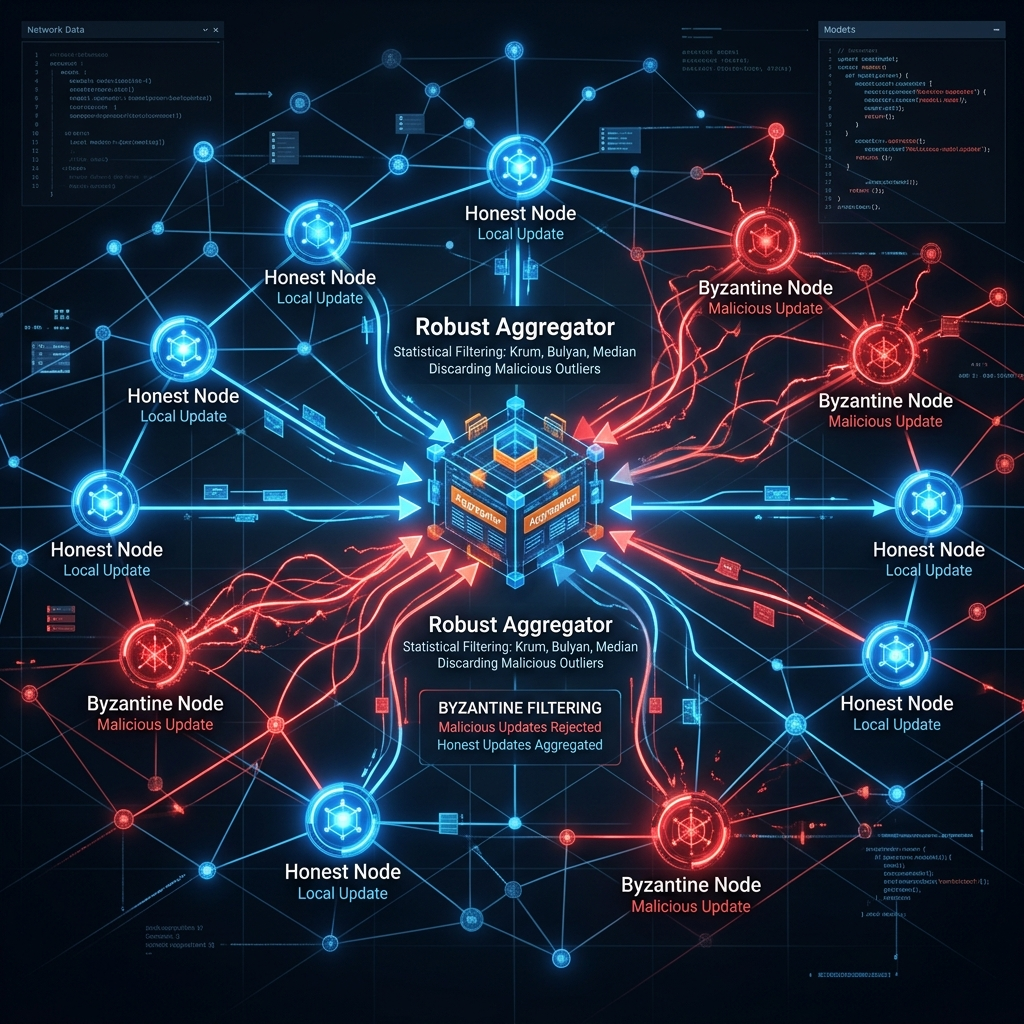
\includegraphics[width=\textwidth]{figures/ch10_robust.png}
\caption{Robust Aggregation: A network graph showing the filtering of Byzantine (malicious) updates to maintain the integrity of the global model aggregation.}
\label{fig:ch10_robust}
\end{figure}

\subsection{Collusion Attacks and Sybil Nodes}
\label{subsec:collusion_attacks}

Individual Byzantine clients are detectable by geometric distance (Krum) or statistical outlier rules (Trimmed Mean). A more sophisticated adversary deploys \textbf{coordinated Sybil nodes}: a group of $f$ colluding clients that each send individually plausible updates, but whose \emph{combined} effect steers the global model toward the attacker's objective.

\textbf{Why simple rules fail against collusion.} Coordinate-Wise Trimmed Mean clips the $\beta$ most extreme values per coordinate. If $f > \beta$ colluding clients each contribute a moderate-magnitude poisoned gradient, every individual update stays within the trimming window — yet their aggregate effect corrupts the model. Krum selects the single lowest-score update; $f$ colluding clients can pre-arrange their updates so that each Sybil appears as the "most typical'' member of the group, displacing honest updates from the selection set.

\textbf{Identity-Verified FL with Decentralized Identifiers (DIDs).} The architectural countermeasure is to break the pseudonymous identity assumption that enables Sybil attacks. \textbf{Decentralized Identifiers (DIDs)} (discussed in Chapter~\ref{chap:decentralized_identity}) bind each FL participant to a cryptographically verifiable, non-transferable identity credential anchored to a consortium blockchain. This enables three anti-Sybil properties:

\begin{description}
  \item[One-DID-per-client enforcement:] The aggregator rejects updates not accompanied by a valid DID Verifiable Presentation. An adversary cannot register multiple identities without acquiring multiple distinct hardware attestation credentials (SGX quotes or ARM TrustZone certificates), raising the cost of a Sybil attack from near-zero to near-hardware-acquisition cost.
  \item[Stake-weighted reputation:] Each DID accumulates a gradient-quality reputation score across rounds. Low-reputation DIDs have their updates discounted; a new DID starts with minimum weight, preventing a fresh Sybil from immediately influencing the model.
  \item[Audit trail without deanonymization:] The DID is pseudonymous — the aggregator knows the DID, not the hospital or user behind it. On-chain commitments record which DID submitted which round's update hash, enabling post-incident forensics without exposing the client's identity.
\end{description}

\begin{svgraybox}
\textbf{Sybil Resistance in Practice:} A consortium of ten Vietnamese hospitals participating in a federated diagnostic AI is required under Decree 13 to maintain an audit log of data processors. The DID-based FL architecture satisfies this requirement while preventing any single participant from creating phantom identities. The Ministry of Health acts as the DID root-of-trust authority, issuing verifiable credentials to each licensed institution --- a natural extension of the existing healthcare licensing infrastructure.
\end{svgraybox}

\section{Robust Aggregation Rules}
\label{sec:aggregation_rules}

To survive these attacks, the Trustworthy AI Architect must replace the standard simple average (FedAvg) with robust aggregation rules that can filter or penalize outliers.

\paragraph{1. Coordinate-Wise Trimmed Mean} works by sorting the updates received from all clients for each coordinate of the model and discarding the $\beta$ largest and $\beta$ smallest values before computing the average. This prevents a single client from pulling the global model in a specific direction using extreme gradient values.

\paragraph{2. Krum (Distance-Based Selection)} selects a single "best" update based on its distance to its neighbors. For each update $w_i$, the server calculates a score:
\begin{equation}
\text{Score}(i) = \sum_{j \in \text{Neighbors}(i)} \|w_i - w_j\|^2
\end{equation}
The update with the lowest score (the one most typical of the group) is selected as the global update for that round.

\section{The Privacy-Robustness Conflict}
\label{sec:privacy_robustness_conflict}

\begin{svgraybox}
\textbf{The Architect's Dilemma:} There is a fundamental conflict between \textbf{Secure Aggregation} (which hides individual updates from the server to protect privacy) and \textbf{Robust Aggregation} (which requires the server to inspect or sort individual updates to detect malicious ones). If the updates are cryptographically masked, the server cannot see which one is an outlier. This "Privacy-Integrity'' trade-off is a core area of ongoing research and a critical design decision for any secure distributed system.
\end{svgraybox}

\subsection{Trust Mitigation Matrix: Resolving the Privacy-Integrity Dilemma}
\label{subsec:trust_mitigation_matrix}

The dilemma has no perfect solution, but the architect has a spectrum of approaches that trade off between robustness strength, privacy preservation, and operational cost. Table~\ref{tab:trust_mitigation_matrix} maps five architectural strategies across these axes.

\begin{table}[ht]
\centering
\caption{Trust Mitigation Matrix for the Privacy-Robustness conflict in Federated Learning. Robustness strength is rated relative to adaptive (collusion-aware) adversaries; privacy preservation is rated relative to individual gradient exposure.}
\label{tab:trust_mitigation_matrix}
\renewcommand{\arraystretch}{1.3}
\begin{tabular}{p{3.0cm} p{3.2cm} p{1.6cm} p{1.6cm} p{2.4cm}}
\hline\noalign{\smallskip}
\textbf{Strategy} & \textbf{Mechanism} & \textbf{Robustness} & \textbf{Privacy} & \textbf{Overhead} \\
\noalign{\smallskip}\svhline\noalign{\smallskip}
Plaintext Krum / Trimmed Mean & Server inspects raw gradients; applies robust rule & High & \cellcolor{costhigh}None & Low \\[3pt]
SecAgg only & Pairwise masking; server sees only aggregate & None & \cellcolor{costlow}Full & Medium \\[3pt]
\textbf{ZK-Proof of Gradient Norm} & Client proves $\|\mathbf{g}_i\|_2 \leq C$ without revealing $\mathbf{g}_i$; server rejects norm-violating updates & Medium & \cellcolor{costlow}Full & \cellcolor{costhigh}High (ZK circuit) \\[3pt]
\textbf{Commitment + Selective Reveal} & Client commits $h = \mathrm{SHA256}(\mathbf{g}_i)$; reveals only on anomaly flag & Medium & \cellcolor{costmed}Conditional & Low--Med \\[3pt]
\textbf{TEE-based Aggregator} & Secure enclave runs Krum on decrypted updates; OS never sees individual gradients & \cellcolor{costlow}High & \cellcolor{costlow}High & Medium \\
\noalign{\smallskip}\hline\noalign{\smallskip}
\end{tabular}
\end{table}

\textbf{ZK-Proof of Gradient Norm} is the theoretically cleanest approach: the client constructs a zero-knowledge proof that their gradient norm satisfies $\|\mathbf{g}_i\|_2 \leq C$ (the DP-SGD clipping bound), without revealing any coordinate of $\mathbf{g}_i$. The server can reject any update whose proof fails, blocking extreme outliers while the cryptographic mask keeps the content private. The practical challenge is proof generation time: current ZK-SNARK circuits for 100K-dimensional gradient vectors require several seconds per round --- feasible for hourly hospital batch FL, but too slow for real-time edge deployments.

\textbf{TEE-based Aggregation} (the shaded row) is the most deployment-ready solution for 2025--2026: the server runs the Krum filter inside an Intel SGX or AWS Nitro Enclave. Decrypted gradients exist only inside the enclave's protected memory; the host OS sees only the filtered aggregate. This is the approach used in the Full-Stack Blueprint of Section~\ref{sec:blueprint_federated_fraud}.

% ------------------------------------------------------------------
\section{Full-Stack Blueprint: Cross-Border Federated Fraud Detection}
\label{sec:blueprint_federated_fraud}
% ------------------------------------------------------------------

To conclude Part III, we synthesize the four Secure Distributed Systems pillars---Federated Learning, Secure Aggregation, Hardware-Rooted Trust, and Robust Aggregation---into a single \textbf{Full-Stack Blueprint} for a Southeast Asian bank consortium building a shared fraud detection model without pooling customer transaction data.

In this architecture, each bank operates a \textbf{TEE-protected FL client} (Chapter 9), where local gradient updates are computed inside an Intel SGX enclave, ensuring the host bank's own infrastructure cannot observe the raw gradients. Before transmission, each update is processed through a \textbf{Secure Aggregation protocol} combining MPC masking and DP-SGD noise (Chapter 8), so the central server receives only the masked, privacy-calibrated aggregate. The central server then applies \textbf{Byzantine-Krum filtering} (Chapter 10) to discard outlier updates from potentially compromised participants. A \textbf{Central Bank Regulator Audit Interface} (the Alignment Layer) receives a per-round summary of which participants were flagged as anomalies, ensuring human oversight of the distributed learning process without exposing individual bank data.

\begin{figure}[ht]
\centering
\begin{tikzpicture}[
    node distance=1.5cm and 2.6cm,
    font=\small,
    layer_box/.style={draw, rounded corners, inner sep=8pt, text centered, font=\bfseries\small, minimum height=1.2cm},
    align_box/.style={layer_box, fill=purple!10, draw=purple!80!black},
    priv_box/.style={layer_box,  fill=blue!10,   draw=blue!80!black},
    sec_box/.style={layer_box,   fill=red!10,    draw=red!80!black},
    ver_box/.style={layer_box,   fill=green!10,  draw=green!80!black},
    arrow/.style={->, >=stealth, thick, draw=gray!70}
]

\node (tee)    [sec_box, text width=5.8cm]
    {\textbf{1. TEE-Protected FL Clients}\\(Security Layer, Intel SGX)\\
     Local training inside enclave\\(gradients private from host OS)};

\node (secagg) [priv_box, right=2.6cm of tee, text width=5.8cm]
    {\textbf{2. SecAgg + DP-SGD}\\(Privacy Layer)\\
     MPC masking + Gaussian noise\\($\varepsilon{=}3.0$ per round)};

\node (robust) [ver_box, below=1.5cm of secagg, text width=5.8cm]
    {\textbf{3. Byzantine-Krum Filter}\\(Verifiability Layer)\\
     Outlier gradient rejection\\(Trimmed Mean fallback)};

\node (reg)    [align_box, below=1.5cm of tee, text width=5.8cm]
    {\textbf{4. Central Bank Audit Interface}\\(Alignment Layer)\\
     Per-round anomaly report\\(human regulator oversight)};

\draw [arrow] (tee.east)    -- node[above, font=\scriptsize] {Masked updates} (secagg.west);
\draw [arrow] (secagg.south)-- node[right, font=\scriptsize] {Aggregated gradient} (robust.north);
\draw [arrow] (robust.west) -- node[above, font=\scriptsize] {Anomaly flags} (reg.east);
\draw [arrow] (tee.south)   -- node[left,  font=\scriptsize] {Round report} (reg.north);

\end{tikzpicture}
\caption{Full-Stack Blueprint (Part III): A cross-border federated fraud detection network integrating TEE-protected client training (Security), DP-SGD + SecAgg privacy (Privacy), Byzantine-Krum outlier filtering (Verifiability), and a Central Bank audit interface (Alignment).}
\label{fig:blueprint_federated_fraud}
\end{figure}

\section{Conclusion}
\label{sec:conclusion_robustness}

Part III has transitioned us from single-point data defense into the complex world of Secure Distributed Systems. We have moved from simple Federated Learning (Chapter 7) toward the cryptographic protection of updates (Chapter 8), hardware-rooted trust (Chapter 9), and Byzantine-resistant aggregation (Chapter 10). 

With these distributed foundations in place, we move into Part IV, which shifts the focus to the internal properties of the models themselves: \textbf{Model Robustness \& Transparency}.


